\documentclass[letterpaper,11pt]{article}


\usepackage{url}
\usepackage{parskip} 	

%other packages for formatting
\RequirePackage{color}
\RequirePackage{graphicx}
\usepackage[usenames,dvipsnames]{xcolor}
\usepackage[scale=0.9]{geometry}


%tabularx environment
\usepackage{tabularx}

%for lists within experience section
\usepackage{enumitem}

% centered version of 'X' col. type
\newcolumntype{C}{>{\centering\arraybackslash}X} 

%to prevent spillover of tabular into next pages
\usepackage{supertabular}
\usepackage{tabularx}
\newlength{\fullcollw}
\setlength{\fullcollw}{0.47\textwidth}

%custom \section
\usepackage{titlesec}				
\usepackage{multicol}
\usepackage{multirow}

%CV Sections inspired by: 
%http://stefano.italians.nl/archives/26
\titleformat{\section}{\Large\scshape\raggedright}{}{0em}{}[\titlerule]
\titlespacing{\section}{0pt}{10pt}{10pt}

%for publications
\usepackage[style=authoryear,sorting=ynt, maxbibnames=2]{biblatex}

%Setup hyperref package, and colours for links
\usepackage[unicode, draft=false]{hyperref}
\definecolor{linkcolour}{rgb}{0,0.2,0.6}
\hypersetup{colorlinks,breaklinks,urlcolor=linkcolour,linkcolor=linkcolour}
\addbibresource{citations.bib}
\setlength\bibitemsep{1.2em}

%for social icons
\usepackage{fontawesome5}

%debug page outer frames
%\usepackage{showframe}


%\usepackage{tgadventor}


%---------------------------------------------------------------------------
%	BEGIN DOCUMENT
%---------------------------------------------------------------------------
\newcounter{pubcount}
\begin{document}

% non-numbered pages}
\pagestyle{empty} 

% \begin{center}
% {\Large Morgan Stanley}
% \end{center}

%---------------------------------------------------------------------------
%	TITLE
%---------------------------------------------------------------------------

% \begin{tabularx}{\linewidth}{ @{}X X@{} }
% \huge{Your Name}\vspace{2pt} & \hfill \emoji{incoming-envelope} email@email.com \\
% \raisebox{-0.05\height}\faGithub\ username \ | \
% \raisebox{-0.00\height}\faLinkedin\ username \ | \ \raisebox{-0.05\height}\faGlobe \ mysite.com  & \hfill \emoji{calling} number
% \end{tabularx}
% \begin{minipage}{0.15\textwidth} % Adjust width to your desired photo size
%     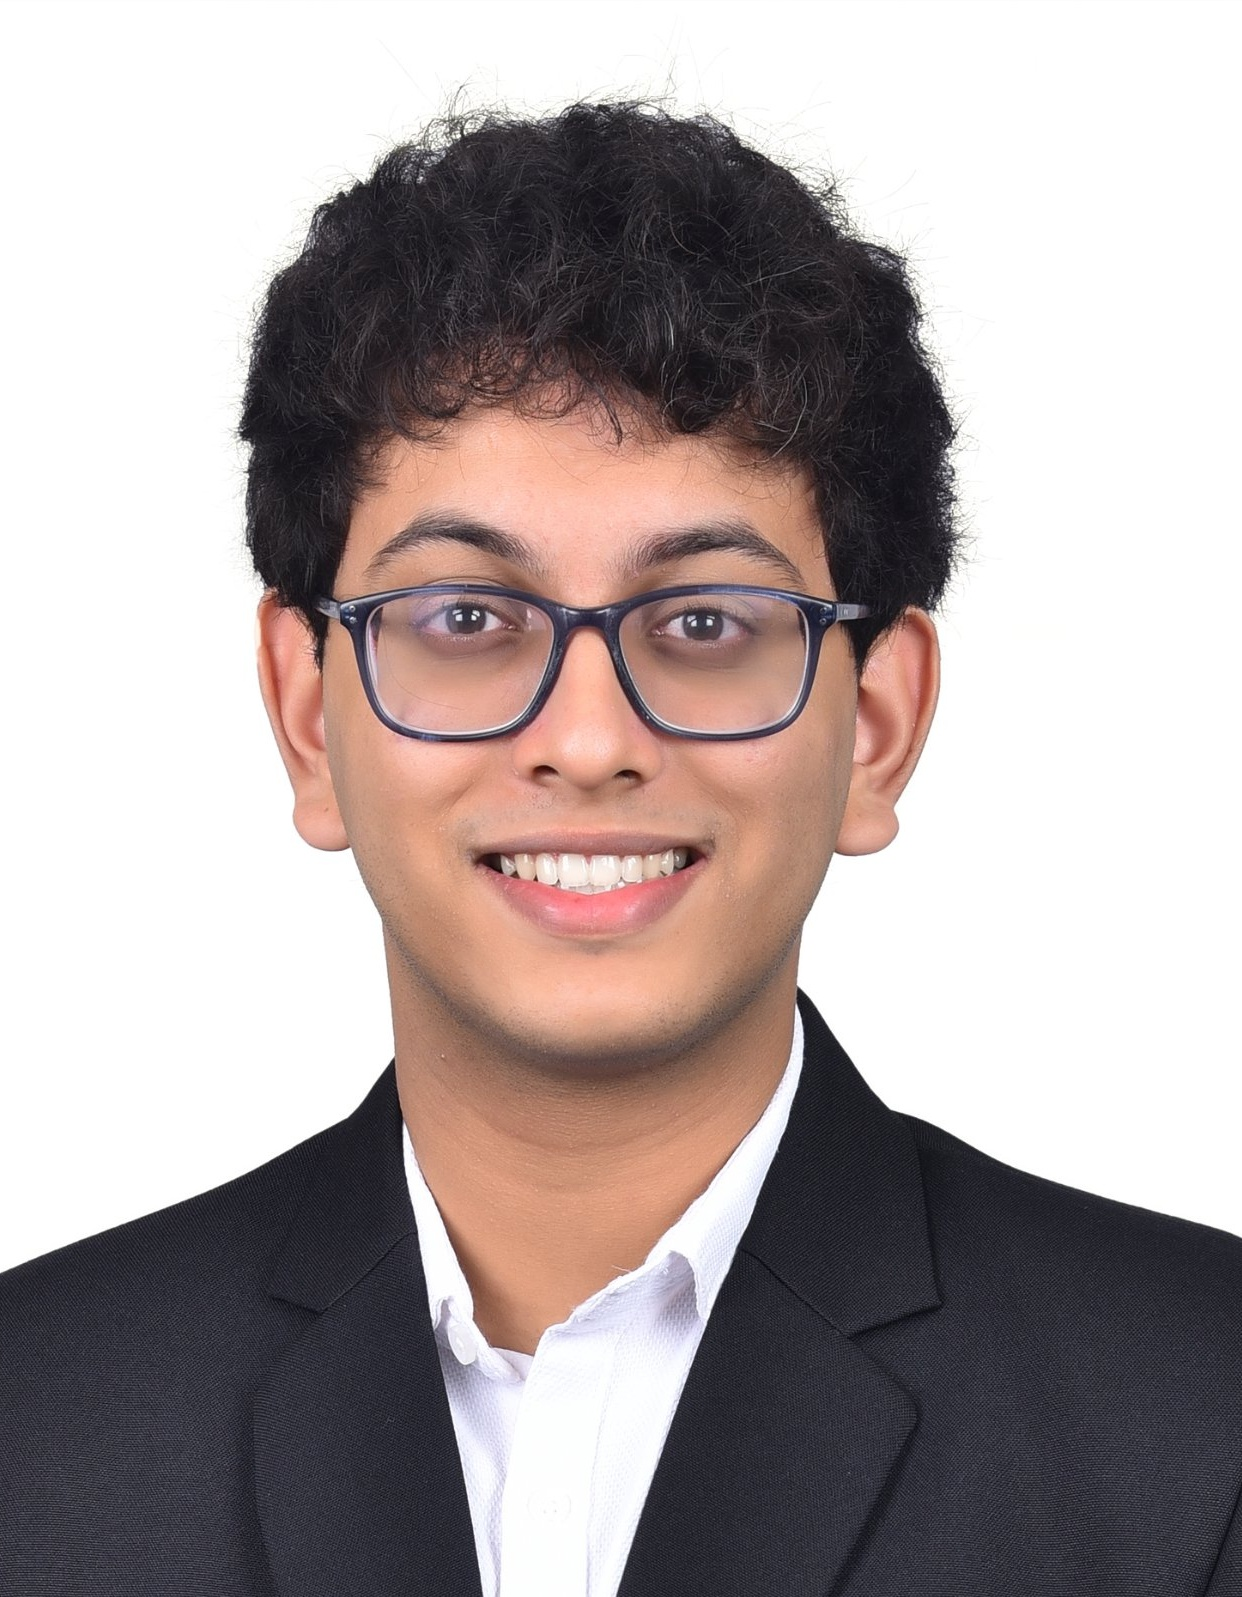
\includegraphics[width=0.8\linewidth]{photo.jpg} % Path to your photo
% \end{minipage}%
% \hspace{0.05\textwidth} % Space between the photo and text
% \begin{minipage}{0.6\textwidth}
%     % \raggedright
%     \centering % Center the text
%     \textbf{\huge SOHAM WALIMBE} \\[7.5pt]
%     \large % Adjust font size
%     \href{https://www.linkedin.com/in/soham-walimbe-41ba49247/}{\raisebox{-0.05\height}\faLinkedin\ LinkedIn} \ $|$ \  
%     \href{mailto:sohamwalimbe15@gmail.com}{\raisebox{-0.05\height}\faEnvelope \ Email} \ $|$ \ 
%     \href{tel:+91 7218347988}{\raisebox{-0.05\height}\faMobile \ +91 7218347988}
% \end{minipage}

% \begin{center} % Center the entire block
%     \begin{minipage}{0.9\textwidth} % Controls the width of the content block
%         \begin{minipage}{0.15\textwidth} % Size for the photo
%             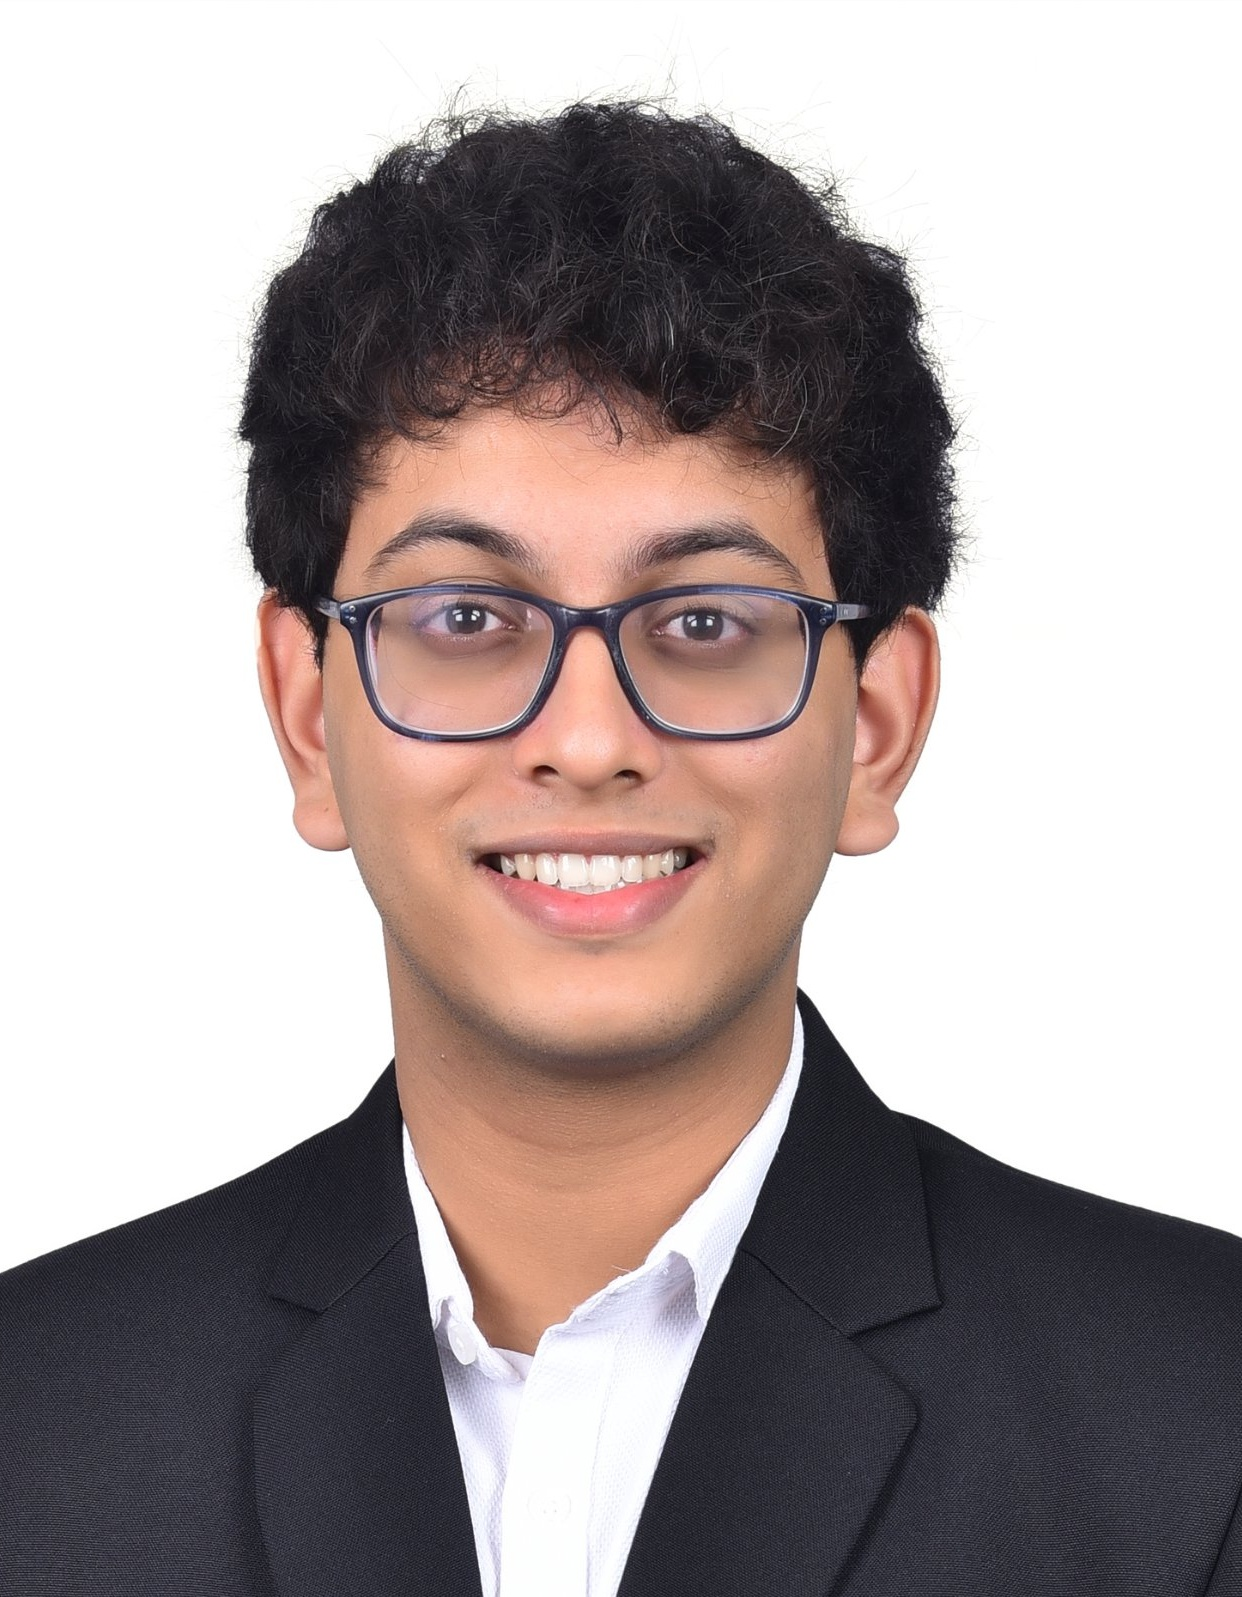
\includegraphics[width=\linewidth]{photo.jpg} % Your photo here
%         \end{minipage}%
%         \hspace{0.05\textwidth} % Space between the photo and text
%         \begin{minipage}{0.75\textwidth}
%             \centering % Left-align the text inside this block
%             \textbf{\Huge SOHAM WALIMBE} \\[7.5pt]
%             \large % Larger font for contact info
%             \href{https://www.linkedin.com/in/soham-walimbe-41ba49247/}{\raisebox{-0.05\height}\faLinkedin\ LinkedIn} \ $|$ \  
%             \href{mailto:sohamwalimbe15@gmail.com}{\raisebox{-0.05\height}\faEnvelope \ Email} \ $|$ \ 
%             \href{tel:+91 7218347988}{\raisebox{-0.05\height}\faMobile \ +91 7218347988}
%         \end{minipage}
%     \end{minipage}
% \end{center}


\begin{tabularx}{\linewidth}{@{} C @{}}
\Huge{SOHAM WALIMBE} \\[7.5pt]
\href{https://github.com/Sohamwalimbe}{\raisebox{-0.05\height}\faGithub\ GitHub} \ $|$ \
% TODO: add Google Scholar URL, then uncomment
% \href{https://scholar.google.com/citations?user=XXXX}{\raisebox{-0.05\height}\faGraduationCap\ Scholar} \ $|$ \
% TODO: add personal website URL, then uncomment
% \href{https://your-site.com}{\raisebox{-0.05\height}\faGlobe\ Website} \ $|$ \
\href{https://www.linkedin.com/in/soham-walimbe-41ba49247/}{\raisebox{-0.05\height}\faLinkedin\ LinkedIn} \ $|$ \  
\href{mailto:sohamwalimbe15@gmail.com}{\raisebox{-0.05\height}\faEnvelope \ Email} \ $|$ \ 
\href{tel:+91 7218347988}{\raisebox{-0.05\height}\faMobile \ +91 7218347988} \\
\end{tabularx}

% \vspace{-0.65em} 
% \section{Summary}
% \vspace{-0.4em} 
% I am a BE ECE student with a Minor in Data Science at BITS Pilani, Goa Campus. Interests: Artificial Intelligence, Cognitive Neuroscience, Machine Learning, Data Science.

% \vspace{-0.5em}


%	EDUCATION
%---------------------------------------------------------------------------\section{Education}
%\vspace{-0.5em} 
\vspace{0.3em}
\section{Education} 
% \vspace{-0.4em} 
\begin{tabularx}{\linewidth}{@{} X@{}}	
    \textbf{Birla Institute of Technology and Science (BITS) Pilani, Goa Campus}  \hfill \textbf{Oct 2021 - Jul 2025} \\
    \textit{Major: Electronics and Communication Engineering  - {\textbf{CGPA: 9.84, Dept. Rank 1}}} \hfill \small\textit{Goa - India} \\
    \textit{Minor: Data Science - \textbf{CGPA: 10/10} } 
\end{tabularx}
% \vspace{-0.3em}





%---------------------------------------------------------------------------
% Experience
%---------------------------------------------------------------------------

\section{Research Experience}

\begin{tabularx}{\linewidth}{ @{}l X@{} }
\textbf{Qure.ai, Bangalore - \textit{AI Scientist}} & \hfill \textbf{Jul 2025 - Present} \\
\end{tabularx}
\vspace{-1.1em}

\textit{qCT: FDA-cleared AI for lung-nodule detection, quantification and characterization in chest CT}
\vspace{-0.5em}
\begin{itemize}
    \item[--] Developed the nodule-growth prediction model for the Lung Nodule Malignancy Score (LNMS); identified label noise as the main bottleneck, motivating a move to external data that raised AUC from 0.58 to 0.76. Co-designed the final LNMS ensemble, which uses these embeddings and is headed for production and a planned FDA Breakthrough Device application.\vspace{-0.5em}
    \item[--] Led development of the false-positive reduction model for the FDA-cleared detection pipeline, raising precision by $\sim$15 points (TODO: X\% $\rightarrow$ Y\%) at unchanged recall (TODO: Z\%).\vspace{-0.5em}
    \item[--] Improved nodule measurement: raised Dice on large nodules ($>$30 mm) from $\sim$0.25 to 0.70 with a training-free resampling strategy, brought diameter error to 0.8 mm MAE, and devised a training-free diffusion-filtering and k-means method to separate the solid and ground-glass components of part-solid nodules.\vspace{-0.5em}
    \item[--] Trained an orientation- and size-invariant lobe segmentation model with constant inference time, making several production modules for scan reorientation and slice categorization obsolete.\vspace{-0.5em}
    \item[--] Designed the rules and pipelines of a large-scale nodule data framework that matches radiology reports to detections, deriving nodule-level ground truth and hard negatives from $\sim$400k CTs and nodule-level labels from patient- and lobe-level annotations for LNMS; served as the point of contact for product and engineering teams on it.\vspace{-0.5em}
    \item[--] Also contributed to self-supervised CT pretraining (DINO, MAE, Pixio; $\sim$250k CTs) and ad hoc analyses for FDA submissions.
\end{itemize}
% Numbers pending manager approval for public sharing

\vspace{0.6em}

\begin{tabularx}{\linewidth}{ @{}l X@{} }
\textbf{CAMMA, University of Strasbourg, CNRS - \textit{Research Intern}} & \hfill \textbf{Jul 2024 - Dec 2024} \\
\end{tabularx}
\vspace{-1.1em}

\textbf{Bachelor's Thesis:} \textit{Adaptation of Multi-modal Representation Models for Multi-Task Surgical Computer Vision} \\
Supervisors: Dr. Britty Baby, Prof. Nicolas Padoy
\vspace{-0.5em}
\begin{itemize}
    \item[--] Developed MML-SurgAdapt, a unified multi-task framework that adapts CLIP through natural-language supervision to perform surgical phase recognition, action-triplet recognition and Critical View of Safety (CVS) assessment in laparoscopic cholecystectomy (Cholec80, Endoscapes2023, CholecT50).\vspace{-0.5em}
    \item[--] Extended Single Positive Multi-Label (SPML) learning to train on partially annotated data across tasks, its first use for integrating multiple surgical tasks; one model performed comparably to task-specific models (74.16 F1 phase, 30.32 mAP triplets, 55.88 mAP CVS).\vspace{-0.5em}
    \item[--] Published as first author at MICCAI 2025 [1], with code released publicly; nominated for the Best Paper and Young Scientist Awards.
\end{itemize}
\vspace{0.1em}

\textbf{Project:} \textit{CoSimGen: Controllable Diffusion Model for Simultaneous Image and Segmentation Mask Generation} \\
Supervisor: Mr. Rupak Bose
\vspace{-0.5em}
\begin{itemize}
    \item[--] Ran the full quantitative evaluation of CoSimGen [2], a controllable diffusion model that jointly generates images and their segmentation masks, benchmarking it against 4 generative baselines (GANs, VAE, diffusion) across 5 datasets on 6 metrics, including FID, KID, LPIPS and Inception Score.
\end{itemize}

\vspace{0.6em}

\begin{tabularx}{\linewidth}{ @{}l X@{} }
\textbf{CSIR-CEERI, Pilani - \textit{Machine Learning Research Intern}} & \hfill \textbf{May 2023 - Jul 2023} \\
Supervisor: Dr. Dhiraj Sangwan
\end{tabularx}
\vspace{-1.2em}

\begin{itemize}
    \item[--] Implemented an unsupervised anomaly segmentation framework that flags contraband (e.g., guns, knives) in baggage X-rays from UNet reconstruction errors, trained only on normal scans.\vspace{-0.5em}
    \item[--] Clustered anomalous regions into instances with bounding boxes and labels, turning anomaly maps into object detections for airport security screening.\vspace{-0.5em}
    \item[--] Applied Gaussian-Weighted Fourier Stylization (GW-FS) during training and inference to suppress scanner-specific appearance, improving zero-shot detection when trained on one X-ray dataset and tested on four unseen ones.
\end{itemize}

%---------------------------------------------------------------------------
% Publications
%---------------------------------------------------------------------------
\section{Publications}
% Mark your own name in bold; * = equal contribution. Numbering continues across groups.
\textbf{Published} \vspace{-0.4em}
\begin{enumerate}[label={[\arabic*]}, leftmargin=*, itemsep=0.2em]
    \item \textbf{S. Walimbe}, B. Baby, V. Srivastav, N. Padoy. \textit{Adaptation of Multi-modal Representation Models for Multi-Task Surgical Computer Vision.} MICCAI 2025. \href{https://arxiv.org/abs/2507.05020}{arXiv:2507.05020}. \textbf{Best Paper \& Young Scientist Award nominee.}
\setcounter{pubcount}{\value{enumi}}
\end{enumerate}
\textbf{Preprints} \vspace{-0.4em}
\begin{enumerate}[label={[\arabic*]}, leftmargin=*, itemsep=0.2em]
\setcounter{enumi}{\value{pubcount}}
    \item R. Bose, C. Nwoye, A. Bhat, \textbf{S. Walimbe}, N. Padoy. \textit{CoSimGen: Controllable Diffusion Model for Simultaneous Image and Segmentation Mask Generation.} Preprint, \href{https://openreview.net/forum?id=z8rQHF8OOt}{OpenReview}, 2025. % do not cite as CVPR: not accepted
\setcounter{pubcount}{\value{enumi}}
\end{enumerate}
% \textbf{Under Review} \vspace{-0.4em}   % re-enable when something is submitted
% \begin{enumerate}[label={[\arabic*]}, leftmargin=*, itemsep=0.2em]
% \setcounter{enumi}{\value{pubcount}}
%     \item ...
% \setcounter{pubcount}{\value{enumi}}
% \end{enumerate}
\textbf{In Preparation} \vspace{-0.4em}
\begin{enumerate}[label={[\arabic*]}, leftmargin=*, itemsep=0.2em]
\setcounter{enumi}{\value{pubcount}}
    \item TODO authors. \textit{TODO: geospatial journal paper title.} Journal manuscript in preparation. % move to Under Review once submitted
    \item TODO authors. \textit{TODO: Lung Nodule Malignancy Score (LNMS) paper title.} Journal manuscript in preparation. % targets: The Lancet / Nature Medicine
    \item \textbf{S. Walimbe}, TODO co-authors. \textit{Learned On-Board SAR Compression with Complex-Valued Networks.} In preparation. % TODO: venue once decided
\end{enumerate}

%---------------------------------------------------------------------------
% Research Projects (supervised, non-employment research)
%---------------------------------------------------------------------------
\section{Research Projects}

\begin{tabularx}{\linewidth}{ @{}l X@{} }
\textbf{Learned On-Board Compression of SAR Data with Complex-Valued Networks} & \hfill \textbf{May 2026 - Present} \\
Mentor: Mr. Rupak Bose
\end{tabularx}
\vspace{-1.2em}
\begin{itemize}
    \item[--] Developing a learned compression system for satellite SAR single-look complex (SLC) data: an on-board encoder maps each image to a fixed 2048-value code (64$\times$ fewer values) for downlink, and the ground station reconstructs amplitude and phase.\vspace{-0.5em}
    \item[--] Built real-valued and complex-valued hierarchical autoencoders, plus a conditional flow-matching decoder that samples high-frequency detail lost in compression on the ground at no extra bit cost; the experiment design isolates the effects of complex-valued modelling and of generative decoding.\vspace{-0.5em}
    \item[--] Built the data pipeline (log-compressed complex input that inverts exactly to amplitude and phase) and an evaluation suite of pixel and phase metrics plus Segment Anything (SAM) agreement on amplitude; the complex encoder uses half the parameters of the baseline (57M vs.\ 113M), relevant for on-board hardware.
    % TODO: add results once full-size training runs (compare against a parameter-matched baseline)
\end{itemize}
\vspace{0.3em}

\begin{tabularx}{\linewidth}{ @{}l X@{} }
\textbf{Neural Datacube for Geospatial Data Discovery and Compression} & \hfill \textbf{TODO} \\
Mentor: Mr. Rupak Bose
\end{tabularx}
\vspace{-1.2em}
\begin{itemize}
    \item[--] Designed and developed a NeRF-inspired neural architecture achieving 20$\times$ compression of multispectral satellite imagery. \vspace{-0.5em} % TODO: confirm sensor (Sentinel-1 is SAR, Sentinel-2 is multispectral)
    \item[--] Developed a continuous spatiotemporal representation framework enabling data reconstruction and sampling at arbitrary spatial resolutions for flexible spatiotemporal queries. \vspace{-0.5em}
    \item[--] Optimized model execution by addressing CUDA graph compatibility bottlenecks and deploying the model for edge inference using ONNX Runtime. \vspace{-0.5em}
    \item[--] Explored applications in gradient-based change detection and geospatial feature discovery across spatiotemporal queries.
\end{itemize}
\vspace{0.3em}


\begin{tabularx}{\linewidth}{ @{}l X@{} }
\textbf{Analog Spiking Neural Network for Unsupervised Compression} & \hfill \textbf{Aug 2023 - May 2024}  \\
Guide: Dr. Abhijit Pethe, BITS Pilani, Goa Campus
\end{tabularx}
\vspace{-1.2em}
\begin{itemize}
    \item[--] Built an unsupervised spiking network in which rate-coded inputs drive leaky integrate-and-fire (LIF) neuron circuits through STDP-learning synapse circuits with excitatory and inhibitory connections; the firing rates of $\sim$100 output neurons form a compressed representation of each input. \vspace{-0.5em}
    \item[--] Designed and characterized the neuron and synapse circuits in Cadence Virtuoso under noise and environmental variation, extracted their parameters into behavioral models, and simulated the full network in Python (Brian2).\vspace{-0.5em}
    \item[--] Evaluated the compressed codes with a simple classifier head, reaching 94.76\% accuracy on MNIST from 100 output rates (vs.\ 784 input pixels), and analyzed noise impact and power efficiency.
\end{itemize}

\section{Projects}

\begin{tabularx}{\linewidth}{ @{}X r@{} }
\textbf{Push-T Imitation Learning: Diffusion and Uncertainty-Aware Policies} % TODO: \href{GITHUB-URL}{\faGithub}
 & \textit{\small PyTorch} \\
\end{tabularx}
\vspace{-1.2em}
\begin{itemize}
    \item[--] Built four policies from scratch on a shared ResNet-18 + transformer backbone, trained on 206 human demonstrations: an action-chunking transformer (ACT) baseline, a DDPM diffusion policy with DDIM sampling, and two uncertainty-aware policies (masked diffusion with per-step Gaussian outputs, and a causally masked autoregressive Gaussian policy).\vspace{-0.5em}
    \item[--] Designed the masked-diffusion policy to predict a mean and variance for each future action, trained with negative log-likelihood and decoded by committing the lowest-variance steps first; added a $K$-component mixture head for multimodal demonstrations.\vspace{-0.5em}
    \item[--] Evaluated all policies on the same TODO:N simulator seeds with paired comparisons: the best reached TODO:X mean coverage reward vs.\ TODO:Y for ACT. Measured uncertainty calibration against held-out error and sampled-chunk spread; TODO: finding.\vspace{-0.5em}
    \item[--] Stress-tested robustness to three visual distribution shifts (triangle goal marker, recoloured goal, two T goals) via a custom simulator wrapper; TODO: finding.
\end{itemize}
\vspace{-0.2em}

\begin{tabularx}{\linewidth}{ @{}X r@{} }
\textbf{Masked-Diffusion Speech Recognition (LLaDA-style)} % TODO: \href{GITHUB-URL}{\faGithub}
 & \textit{\small PyTorch, Hugging Face, FastAPI} \\
\end{tabularx}
\vspace{-1.2em}
\begin{itemize}
    \item[--] Designed and trained from scratch a 15M-parameter masked-diffusion transformer decoder that conditions on frozen Whisper-base encoder features and generates transcripts by iterative unmasking, using a LLaDA-style $1/t$-weighted objective on $\sim$60 h of LibriSpeech (under one GPU-hour).\vspace{-0.5em}
    \item[--] Showed that WER falls steadily with more confidence-based decoding steps: 31.3\% $\rightarrow$ 20.8\% on test-clean (8 $\rightarrow$ 128 steps) and 42.2\% $\rightarrow$ 32.3\% on test-other (8 $\rightarrow$ 64 steps), vs.\ $\sim$54\% for one-shot parallel decoding.\vspace{-0.5em}
    \item[--] Error analysis showed $\sim$73\% of word errors were substitutions, mostly near-miss spellings from composing BPE pieces without a language model, pointing to decoder capacity and text data rather than acoustics as the bottleneck.\vspace{-0.5em}
    \item[--] Shipped a CPU-only web demo that replays the decoding trajectory step by step, highlights word-level errors on test clips, and transcribes uploaded audio.
\end{itemize}
\vspace{-0.2em}

\begin{tabularx}{\linewidth}{ @{}X r@{} }
\textbf{3D Point Cloud Segmentation from Scratch} % TODO: \href{GITHUB-URL}{\faGithub}
 & \textit{\small PyTorch, NumPy} \\
\end{tabularx}
\vspace{-1.2em}
\begin{itemize}
    \item[--] Built an end-to-end part and scene segmentation pipeline with no point-cloud libraries and implemented PointNet with input and feature T-Nets, reaching 0.807 instance mIoU on ShapeNetPart (0.801 without category labels); traced the weakest results to rare parts with under 0.1\% of training points.\vspace{-0.5em}
    \item[--] Swept input size from 128 to 4096 points: instance mIoU stayed within $\sim$0.3 points from 512 to 4096, while 512 points gave $\sim$4$\times$ the batch throughput of 2048.\vspace{-0.5em}
    \item[--] Extended PointNet with heteroscedastic aleatoric uncertainty (learned per-point logit noise, Monte Carlo likelihood), preserving accuracy (val.\ 0.837 vs.\ 0.831); the shared $\sigma$ collapsed toward zero and detected errors worse than softmax confidence (AUROC 0.72 vs.\ 0.89). TODO: per-class $\sigma$ result.
    % TODO once done: PointNet++ (FPS, ball query, set abstraction, feature propagation) -> ShapeNetPart mIoU X
    % TODO once done: S3DIS (13 classes, Area 5 held out) -> mIoU X (PointNet) / X (PointNet++)
\end{itemize}
\vspace{-0.2em}

\begin{tabularx}{\linewidth}{ @{}X r@{} }
\textbf{Agent Courtroom: LLM Debate for Scalable Oversight} % TODO: \href{GITHUB-URL}{\faGithub}
 & \textit{\small Python, asyncio, FastAPI} \\
\end{tabularx}
\vspace{-1.2em}
\begin{itemize}
    \item[--] Implemented the Khan et al.\ (2024) debate setup as an async pipeline: strong-model debaters argue assigned answers to long-passage QuALITY questions and a weaker judge sees only the transcript, across four conditions (judge alone, consultancy, debate, and a passage-access upper bound).\vspace{-0.5em}
    \item[--] Added quote verification that flags fabricated evidence to the judge, and a statistics suite: bootstrap CIs, exact McNemar test, Brier score with reliability plots, a position-bias test, and ablations over rounds, quote verification and judge size.\vspace{-0.5em}
    \item[--] Shipped a live demo in which a clerk agent retrieves Wikipedia sources and two debaters argue a user-given topic before a source-blind judge, streamed over SSE; all runs are cached, resumable and held to a hard spend cap.
    % TODO: add a results line only after real dev/test runs
\end{itemize}
\vspace{-0.2em}

\begin{tabularx}{\linewidth}{ @{}X r@{} }
\textbf{Prompt-Injection Arena: Defense Benchmark and Public Attack Game} % TODO: \href{GITHUB-URL}{\faGithub}
 & \textit{\small Python, asyncio, FastAPI, SQLite} \\
\end{tabularx}
\vspace{-1.2em}
\begin{itemize}
    \item[--] Built a benchmark measuring how five layered defenses, from a plain system prompt (L0) to privilege separation with a quarantined no-tool reader (L4), protect a sandboxed tool-using agent; attack success is scored by a deterministic code judge, not a model.\vspace{-0.5em}
    \item[--] Assembled 250 labeled attacks (direct and indirect, 17 technique tags, incl.\ 50 from Tensor Trust) with a fixed train/test split, 41 benign tasks to measure utility, and an adaptive LLM red-team agent; analysis via Wilson CIs, per-technique breakdowns, ablations and a security--utility tradeoff.\vspace{-0.5em}
    \item[--] Wrote the run infrastructure without agent frameworks (cached, resumable, budget-capped runs routed across Anthropic, free APIs and Ollama) and shipped a public web game with a leaderboard and rate limiting.
    % TODO: add a results line (e.g. L4 attack-success reduction) only after real runs
\end{itemize}
\vspace{-0.2em}

%---------------------------------------------------------------------------
% Teaching
%---------------------------------------------------------------------------
\section{Teaching Experience}

\begin{tabularx}{\linewidth}{ @{}l X@{} }
\textbf{Machine Learning - \textit{Undergraduate Teaching Assistant}} & \hfill \textbf{Jan 2025 - May 2025} \\
\end{tabularx}
\vspace{-1.2em}
\begin{itemize}
    \item[--] Designed lab sessions on Naive Bayes, clustering and optimization algorithms (momentum, Adam), and led a tutorial on decision trees and ensemble methods; also helped grade quizzes.
\end{itemize}
\vspace{-0.3em}

\begin{tabularx}{\linewidth}{ @{}l X@{} }
\textbf{Operating Systems - \textit{Undergraduate Teaching Assistant}} & \hfill \textbf{Jan 2025 - May 2025} \\
\end{tabularx}
\vspace{-1.2em}
\begin{itemize}
    \item[--] Designed a lab-based practical exam on processes, forks, threads, shared memory and semaphores, and conducted a tutorial session.
\end{itemize}
\vspace{-0.3em}

\begin{tabularx}{\linewidth}{ @{}l X@{} }
\textbf{Basic Electronics - \textit{Undergraduate Teaching Assistant}} & \hfill \textbf{May 2024 - Jul 2024} \\
\end{tabularx}
\vspace{-1.2em}
\begin{itemize}
    \item[--] Wrote midterm and final exam questions for the online B.Sc. Computer Science programme and supported students through the course discussion forums.
\end{itemize}
\vspace{-0.3em}

\begin{tabularx}{\linewidth}{ @{}l X@{} }
\textbf{Microelectronic Circuits - \textit{Undergraduate Teaching Assistant}} & \hfill \textbf{Jan 2024 - May 2024} \\
\end{tabularx}
\vspace{-1.2em}
\begin{itemize}
    \item[--] Designed lab problems and ran weekly sessions in which students designed transistor amplifier circuits and simulated them in Cadence Virtuoso. \vspace{-0.5em}
    \item[--] Co-created evaluation questions with the course faculty.
\end{itemize}
\vspace{-0.3em}

\begin{tabularx}{\linewidth}{ @{}l X@{} }
\textbf{Digital Design - \textit{Undergraduate Teaching Assistant}} & \hfill \textbf{Aug 2023 - Dec 2023} \\
\end{tabularx}
\vspace{-1.2em}
\begin{itemize}
    \item[--] Ran weekly lab sessions in which students built digital circuits on breadboards using integrated circuits, and helped develop and grade course evaluations.
\end{itemize}
\vspace{-0.3em}

\section{Honors \& Awards}
%\vspace{-0.4em}
\vspace{0.1em}
\begin{itemize}
    \item Nominated for the \textbf{Best Paper Award} and \textbf{Young Scientist Award}, MICCAI 2025.
    \item \textbf{Silver Medal}: ranked 2nd in a graduating batch of 800 students, BITS Pilani, Goa Campus, 2025.
    \item \textbf{Prof. G. Raghurama Outstanding Student Award}, BITS Pilani, Goa Campus, 2025.
    \item \textbf{100\% Merit Scholarship} (full tuition waiver) for 7 semesters, BITS Pilani.
    \item \textbf{IPCD Partial Travel Grant} for bachelor's thesis research at CAMMA, Strasbourg; International Programmes and Collaboration Division, BITS Pilani, 2024.
\end{itemize}
\vspace{-0.4em}

% %---------------------------------------------------------------------------
% %	Test Scores (off by default: scores are reported officially in applications)
% %---------------------------------------------------------------------------
% \section{Test Scores}
% \textbf{GRE:} Quantitative 170/170, Verbal 155/170, AWA 4.0/6.0 \\
% \textbf{TOEFL iBT:} 110/120

%---------------------------------------------------------------------------
%	Skills
%---------------------------------------------------------------------------
\section{Skills}
%\vspace{-0.4em} 
\vspace{0.2em}

\textbf{Languages and Tools:} Python, C, C++, SQL (incl. DuckDB), MATLAB, Git, Linux, Docker, SLURM, \LaTeX \\
\textbf{Deep Learning:} PyTorch (incl. DDP multi-GPU training), PyTorch Lightning, Hugging Face (Transformers, Datasets, PEFT), timm \\
\textbf{Data and Experiment Tracking:} NumPy, SciPy, Pandas, scikit-learn, OpenCV, Matplotlib, Weights \& Biases, ClearML \\
\textbf{Medical Imaging:} MONAI, SimpleITK \\
\textbf{LLMs, Agents and Apps:} Anthropic SDK, LangChain, Ollama, FastAPI, Flask, Gradio, Streamlit \\
\textbf{Methods:} Self-supervised learning (DINO, MAE), diffusion models (DDPM, masked diffusion), vision-language models, 3D medical image segmentation, point cloud learning, LLM evaluation \\
\vspace{-1.5em}

\section{Coursework}
%\vspace{-0.3em}
\vspace{-0.2em}
\textbf{Machine Learning \& AI:} Machine Learning, Reinforcement Learning, Artificial Intelligence, Foundations of Data Science \\
\textbf{Mathematics \& Statistics:} Multivariable Calculus, Linear Algebra \& Complex Analysis, Differential Equations, Probability \& Statistics, Applied Statistical Methods \\
\textbf{Computer Science:} Foundations of Data Structures \& Algorithms, Operating Systems \\
\textbf{Signals \& Information:} Signals \& Systems, Digital Signal Processing, Information Theory \& Coding \\
\textbf{Online (NPTEL):} Theory of Computation, Compiler Design, Discrete Mathematics, Large Language Models, Computer Networks \\
\vspace{-1.4em}
    
  % \small\textit{Courses with an \textbf{A (the highest grade)}} are marked with a ($^*$)
  % \vspace{-1.25em}

%---------------------------------------------------------------------------
%	PORs
%--------------------------------------------------------------------------


\section{Positions of Responsibility}
%\vspace{-0.4em} 
% \vspace{0.3em}
\begin{tabularx}{\linewidth}{ @{}l X@{} }

\textbf{Synchronoise, BITS Goa A Cappella Crew - \textit{Sub-Coordinator}} & \hfill \textbf{May 2023 - Apr 2024 }\\
\end{tabularx}

\begin{itemize}
    \vspace{-0.5em}
    \item[--] Co-led the club as one of its three heads, organizing campus performances and events and managing its finances and logistics. 
\end{itemize}

\begin{tabularx}{\linewidth}{ @{}l X@{} }
\textbf{Nirmaan (NGO), BITS Pilani Goa Chapter - \textit{Crew Member}} & \hfill \textbf{Dec 2022 - May 2024} \\

\end{tabularx}

\begin{itemize}
    \vspace{-0.5em}
    \item[--] Taught mathematics and English to underprivileged children three days a week with the Teach Zari team, and helped provide educational resources to underserved communities. \vspace{-0.5em}
\end{itemize}
\vspace{-0.8em}

% \section{References}
% %\vspace{-0.4em} 
% \vspace{0.2em}

% \textbf{Dr. Abhijit Pethe :}   \normalsize{Associate Professor, BITS Pilani Goa Campus, \href{mailto:abhijitp@goa.bits-pilani.ac.in}{abhijitp@goa.bits-pilani.ac.in}}\\
% \textbf{Dr. Britty Baby :}   \normalsize{Postdoctoral Researcher, CAMMA, University of Strasbourg, \href{mailto:bbaby@unistra.fr}{bbaby@unistra.fr}
% }

% \vspace{-0.35em}

% \begin{tabularx}{\linewidth}{ @{}l X@{} }
%  \textbf{Waves Controls : }Core Member & \hfill \textbf{Sept 2022 - Present} \\

% \end{tabularx}


%---------------------------------------------------------------------------
%	Exams
%--------------------------------------------------------------------------

\end{document}
%---------------------------------------------------------------------------
%	End
%--------------------------------------------------------------------------
